\seite{}{Hybride Systeme}\anchorpage{1}{neu5}{5 · Hybride Systeme, Diskontinuitäten und Ereignissteuerung}\ey{KAPITEL 5}\ptitle{Hybride Systeme, Diskontinuitäten und Ereignissteuerung}
Ein Ball fällt. Zwischen zwei gespeicherten Höhen ist er kurz auf den Boden getroffen und bereits wieder aufgestiegen. Ein Modell, das erst am nächsten Ausgabetakt reagiert, kann Energie gewinnen oder den Stoß ganz übersehen. Wie findet man den Augenblick, in dem das Bewegungsgesetz wechselt?
\subt{Der Weg durch das Kapitel}
{\tblstart\begin{tabularx}{\linewidth}{@{}Yr@{}}\toprule
\hyperlink{abs5-1}{5.1 · Zeit- und Zustandsereignisse} & \pagelink{abs5-1}\\[2pt]
\hyperlink{abs5-2}{5.2 · Nullstellen während eines Schritts} & \pagelink{abs5-2}\\[2pt]
\hyperlink{abs5-3}{5.3 · Reset und Neustart} & \pagelink{abs5-3}\\[2pt]
\hyperlink{abs5-4}{5.4 · Chattering und Zeno-Folgen} & \pagelink{abs5-4}\\[2pt]
\bottomrule\end{tabularx}\par}
\par\vfill{\centering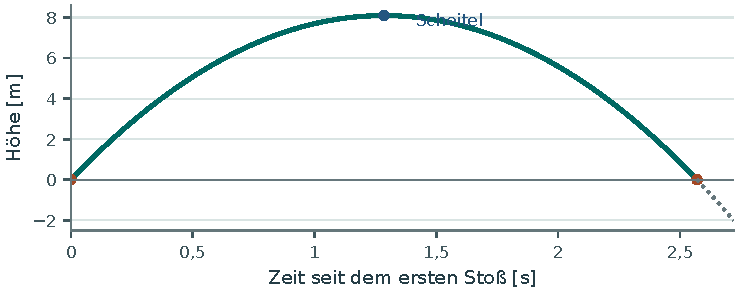
\includegraphics[width=.88\linewidth,height=49mm,keepaspectratio]{ball.pdf}\par}\capline{Jeder glatte Flug endet am gerichteten Kontakt.}
\seite{}{Hybride Systeme}\anchorpage{2}{abs5-1}{5.1 · Zeit- und Zustandsereignisse}\ey{ABSCHNITT 5.1}\ptitle{Zeit- und Zustandsereignisse}
\hypertarget{punkt5-1-1}{}\subt{5.1.1\enspace Welcher Zeitpunkt ist im Voraus bekannt?}
Ein Steuergerät tastet alle zehn Millisekunden ab. Der nächste Takt liegt vor dem Integrationsschritt fest. Wann derselbe Antrieb seinen Anschlag erreicht, hängt von Ort und Geschwindigkeit ab. Planen Sie Kalenderereignisse direkt. Für Zustandsereignisse benötigt man zusätzlich eine Suchregel innerhalb des kontinuierlichen Fluges.
\hypertarget{punkt5-1-2}{}\subt{5.1.2\enspace Wächter, Richtung und Modus}
Ein Bodenwächter lautet \(g(t,y)=q\) mit zulässiger Lage \(q\ge0\). Ein Stoß ist nur für Annäherung, also \(v<0\), aktiv. Derselbe Nullwert unmittelbar nach dem Rückprall darf keinen zweiten Stoß auslösen. Die gerichtete Freigabe und der aktive Modus sind damit Teil des Modells.
\seite{Rechenbeispiel}{Hybride Systeme}\anchorpage{2}{kap7}{Kann eine Schaltung zwischen zwei Messungen verschwinden?}\ptitle{Kann eine Schaltung zwischen zwei Messungen verschwinden?}


\lernziel{Sie können einen Schaltzustand mitführen, eine Ereignisrichtung angeben und erklären, weshalb eine Abfrage nur an Schrittenden Übergänge verpassen kann.}
Eine Routine meldet „kein Ereignis“, weil ihr Signal bei Sekunde 0 und bei Sekunde 1 positiv ist. Sie dürfen einmal dazwischen messen. Zu welchem Zeitpunkt würden Sie messen, um die Meldung an der gezeichneten Kurve zu überprüfen?
\minifig{zweiwurzeln}{37mm}{Ein einziger großer Schritt tastet nur die beiden äußeren Punkte ab. Der zusätzliche Punkt bei einer halben Sekunde liegt auf der anderen Seite der Schwelle.}
\subt{Eine Meldung mit Papier und Bleistift prüfen}
Für den Zahlenwert \(s=t/(1\unitm s)\) sei das Signal \(g=(s-0{,}25)(s-0{,}75)\). An beiden Enden erhalten wir \(+0{,}1875\), in der Mitte \(-0{,}0625\). Wegen der Stetigkeit liegt in jeder Hälfte mindestens eine Nullstelle. Die Faktoren liefern sogar die genauen Zeiten \(0{,}25\) und \(0{,}75\unitm s\).

Soll das Gerät nur beim Eintritt in den negativen Bereich schalten, zählt die erste der beiden Nullstellen. Zur zweiten Zeit verlässt das Signal den Bereich. Ein Ereignis braucht daher auch eine Richtung und eine Regel für das, was anschließend geschieht.
\notebox{Jetzt Sie}{Welche zusätzliche Information braucht ein Thermostat bei genau \(20\,^\circ\mathrm C\), wenn er bei \(19\,^\circ\mathrm C\) einschaltet und bei \(21\,^\circ\mathrm C\) ausschaltet? Prüfen Sie je eine Vorgeschichte von oben und von unten. Der bisherige Schaltzustand entscheidet, ob der Raum jetzt heizt.}

\srcs{\textbf{Kernweg}\enspace\see{hybrid}{Thermostat}\quad\textbf{Vertiefung}\enspace\see{qfehler}{Fehler durch Quantisierung}\quad\see{ueb7}{Selbst prüfen}.}

\lektion{Ein Thermostat als erstes Ereignismodell}{hybrid}{Kernweg}{Hybride Systeme}
\vorhersage{7}{Eine Schaltfunktion ist an beiden Schrittenden positiv. Kann sie dazwischen zweimal das Vorzeichen wechseln?}{kontrolleB}
Bei \(20\,^\circ\mathrm C\) kann dieselbe Heizung gerade ein- oder ausgeschaltet sein. Wir nehmen im warmen Modus eine Rate von \(1\unitm{K/min}\) und im kühlen Modus \(-0{,}5\unitm{K/min}\) an. Bei \(19\,^\circ\mathrm C\) schaltet sie beim Absinken ein, bei \(21\,^\circ\mathrm C\) beim Ansteigen aus. Erst Temperatur und Schaltzustand zusammen reichen zur Vorhersage.
\subt{Fluss, Wächter, Richtung und Übergang}
Im Modus „an“ gilt \(\dot T=1\), im Modus „aus“ \(\dot T=-0{,}5\), mit Zeit in Minuten. Ein \emph{Wächter} ist eine Funktion, deren Nullstelle einen Übergang auslösen kann. Im Heizmodus suchen wir eine steigende Nullstelle von \(T-21\). Der Übergang setzt den Modus auf „aus“ und lässt \(T\) stetig. Im Kühlmodus suchen wir eine fallende Nullstelle von \(T-19\). Die obere und die untere Schwelle verhindern unmittelbares Hin- und Herschalten. Diesen Gedächtniseffekt nennt man Hysterese.

Start bei \(20\,^\circ\mathrm C\), Heizung an. Nach einer Minute sind \(21\,^\circ\mathrm C\) erreicht. Vier Minuten später sind es \(19\,^\circ\mathrm C\), zwei weitere Minuten später erneut \(21\,^\circ\mathrm C\). Startet der gleiche Raum bei derselben Temperatur mit ausgeschalteter Heizung, folgt der erste Übergang schon aus einem anderen Wächter. Die Temperatur allein beschreibt die Zukunft daher nicht vollständig.
\subt{Drei Uhren im Modell}
Ein fester Reglertakt ist vorab bekannt. Die physikalische Schaltzeit ergibt sich aus der aktuellen Bahn. Eine interne Zustandsmeldung eines QSS-Verfahrens entsteht, wenn ein numerisch festgelegter Schwellenabstand erreicht ist. Nur die ersten beiden Zeitarten gehören hier zur technischen Aufgabenstellung.
\notebox{Terminologie}{Der \emph{Reset} ist die Abbildung vom Zustand unmittelbar vor dem Übergang auf den Zustand unmittelbar danach. Er kann Größen unverändert lassen oder sprunghaft ändern. Beim \see{praxisdae}{C07-Stiftpendel am Drehpunktwechsel} springt die Winkelgeschwindigkeit. Aus \(\omega^-=-1\unitm{rad/s}\) wird \(\omega^+=-10/3\unitm{rad/s}\), während die Bahngeschwindigkeit bei \(-1\unitm{m/s}\) bleibt. Beim Kugelstoß springen die Bahngeschwindigkeiten.}

\seite{}{Hybride Systeme}\anchorpage{2}{abs5-2}{5.2 · Nullstellen während eines Schritts}\ey{ABSCHNITT 5.2}\ptitle{Nullstellen während eines Schritts}
\hypertarget{punkt5-2-1}{}\subt{5.2.1\enspace Ein Intervall einklammern}
Ist \(G(t)=g(t,p(t))\) für die dichte Bahn \(p\) stetig und haben die Endpunkte entgegengesetzte Vorzeichen, liegt mindestens eine Nullstelle dazwischen. Monotonie sichert höchstens eine. Ein Vorzeichenwechsel über einen Modussprung besitzt diese Aussagekraft erst nach Trennung der glatten Abschnitte.
\hypertarget{punkt5-2-2}{}\subt{5.2.2\enspace Bisektion, Regula falsi und Brent}
Bei Bisektion berechnet man die Mitte, wertet dort den Wächter aus und behält die Hälfte mit Wechsel. Nach \(k\) Halbierungen misst die Klammer \(h/2^k\). Regula falsi verwendet den Schnittpunkt der Sekante mit der Zeitachse. Brent kombiniert schnelle Interpolation mit einer abgesicherten Halbierung. Das Abbruchmaß ist die verbleibende Zeitbreite. Ist zusätzlich \(|G'|\ge m>0\) belegt, übersetzt sich ein Wächterfehler \(\varepsilon\) in höchstens \(\varepsilon/m\) Zeitfehler bei passend isolierter Wurzel.
\hypertarget{punkt5-2-3}{}\subt{5.2.3\enspace Zwei Durchgänge oder eine tangentiale Berührung}
Der Wächter \((t-1/4)(t-3/4)\) ist am Anfang und Ende von \([0,1]\) positiv. Er hat zwei Nullen. Der Wächter \((t-1/2)^2\) berührt die Null einmal. Beide Fälle entgehen dem bloßen Endpunkttest. Polynomextrema, Unterteilung oder ein physikalisch begründeter Höchstschritt können geeignete Klammern liefern. Eine endliche Stichprobe allein beweist deren Vollständigkeit nicht.
\lektion{Vertiefung · Eine glatte Lösung ohne Taylor-Darstellung}{flach}{Vertiefung}{Hybride Systeme}
Das Ventil der Einleitung hat einen sichtbaren Knick in der Volumenkurve erzeugt. Könnte man immer eine Potenzreihe verwenden, wenn stattdessen alle Ableitungen existieren? Ein von null anlaufender Zufluss beantwortet diese Frage. Zeit und Menge seien hier dimensionslos. Wir betrachten das Anfangswertproblem
\[
 x'(s)=q(s),\quad x(0)=0,\qquad
 q(s)=
 \begin{cases}
 0,&s\le0,\\
 \exp(-1/s^2),&s>0 .
 \end{cases}
\]
\subt{Was alle Ableitungen am Start ergeben}
Für \(s>0\) ist jede Ableitung von \(q\) ein Polynom in \(1/s\) mal \(\exp(-1/s^2)\). Dies folgt durch wiederholtes Ableiten. Alle diese Produkte gehen für \(s\downarrow0\) gegen null, denn \(r^m e^{-r^2}\to0\) für \(r\to\infty\) und jedes feste \(m\). Dasselbe gilt nach Division durch \(s\). Induktion mit dem Differenzenquotienten liefert deshalb \(q^{(j)}(0)=0\) für jede Ordnung \(j\). Von links ist die Funktion ohnehin null.
\subt{Eine Vorhersage und ihr Gegenbeweis}
Die eindeutige Lösung lautet \(x(s)=\int_0^s q(u)\dg u\). Damit verschwinden \(x(0)\) und alle Ableitungen von \(x\) am Start. Die Taylorreihe um null ist also die Nullreihe. Für jedes \(s>0\) integriert man jedoch eine positive Funktion über ein Intervall positiver Länge, folglich ist \(x(s)>0\). Die Reihe stimmt in keiner Umgebung von null mit der Lösung überein. Diese ODE hat eine eindeutige, beliebig oft differenzierbare Lösung und besitzt am Start keine reell-analytische Lösung.
\notebox{Was ein Zeitschritt hier anders macht}{Ein Verfahren, das den Zufluss auch innerhalb eines Schritts auswertet, sieht dort positive Werte. Beginnt die Rechnung sehr nahe bei null, können diese Werte in endlicher Rechengenauigkeit trotzdem auf null runden. Für ein Zahlenziel braucht man einen passenden Zeitbereich und eine Fehlerkontrolle.}
\srcs{\href{https://www.math.ucdavis.edu/~hunter/m125a/intro_analysis_ch6.pdf}{J. K. Hunter, Taylor’s theorem and power series, glatte und analytische Funktionen} · \see{formelgrenze}{Geschalteter Zufluss} · \see{keinpolynom}{Elementare Darstellbarkeit}.}

\seite{}{Hybride Systeme}\anchorpage{2}{abs5-3}{5.3 · Reset und Neustart}\ey{ABSCHNITT 5.3}\ptitle{Reset und Neustart}
\hypertarget{punkt5-3-1}{}\subt{5.3.1\enspace Zustandssprung und Saltationsmatrix}
Beim idealen Stoß ergibt die Stoßzahl \(e\) den Reset \(q^+=0,\ v^+=-e v^-\). Verschieben wir die Anflugbahn ein wenig, verschiebt sich auch die Trefferzeit. Für eine glatte Resetabbildung \(R(t,x)\) und einen isolierten transversalen Übergang transportiert die Saltationsmatrix die lineare Störung über den Stoß:
\[
 \Xi=R_x+\frac{(f^+-R_x f^- -R_t)\,g_x}{g_t+g_x f^-}.
\]
Hier ist \(g_x\) ein Zeilenvektor, \(f^-\) die Geschwindigkeit unmittelbar vorher und \(f^+\) diejenige unmittelbar nachher. Der Nenner ist die Geschwindigkeit durch die Schaltfläche. Eine streifende Berührung verletzt die Herleitungsannahme.
\hypertarget{punkt5-3-2}{}\subt{5.3.2\enspace Welche Historie gelöscht wird}
Die dichte Ausgabe endet am Ereignis. Der Solver übernimmt den linken Grenzwert, wendet den Reset genau einmal an, bestimmt den aktiven Modus und prüft den rechten Grenzwert. BDF-Historie, gespeicherte Endsteigungen und Reglerhistorie gehören zur alten glatten Bahn. Bei QSS verlieren die Prognosen geänderter Komponenten ihre Gültigkeit. Zu loggen sind Ereigniszeit, Richtung, beide Zustände und die neue Moduskennung.
\seite{}{Hybride Systeme}\anchorpage{2}{abs5-4}{5.4 · Chattering und Zeno-Folgen}\ey{ABSCHNITT 5.4}\ptitle{Chattering und Zeno-Folgen}
\hypertarget{punkt5-4-1}{}\subt{5.4.1\enspace Warum ein Schalter flattert}
Hält sich eine Temperatur nahe einer einzigen Schwelle auf, genügt Messrauschen zum mehrfachen Umschalten. Zwei physikalisch begründete Hystereseschwellen schaffen einen Abstand. Bei einem Gleitmodus kann dagegen gerade das schnelle Wechseln auf eine andere Modellierung hinweisen. Ein willkürlicher Mindestabstand verändert die Schaltzeiten und gehört in die Ergebnisbeschreibung.
\hypertarget{punkt5-4-2}{}\subt{5.4.2\enspace Endlich viel Zeit für unendlich viele Stöße}
Fällt ein Ball aus Höhe \(H\), ist die erste Aufprallgeschwindigkeit \(u=\sqrt{2gH}\). Die folgenden Flüge dauern \(2eu/g,\,2e^2u/g,\ldots\). Für \(0<e<1\) beträgt ihre Gesamtdauer \(2eu/[g(1-e)]\). Ist nach einem Aufprall die Aufwärtsgeschwindigkeit \(v_+\), verbleiben noch \(2v_+/[g(1-e)]\). Diese Zeit und die nächste Gipfelhöhe \(v_+^2/(2g)\) erlauben einen dokumentierten Übergang in Ruhe. Endliche Federkontakte verlangen ein anderes Modell.
\werkblatt{5}{Selbst prüfen}{ueb7}{Schalten und Neuplanen}

\merke{Bei einem hybriden Modell gehören zum kontinuierlichen Gesetz auch der aktive Modus, die Übergangsfläche, die Richtung und die neue Ausgangslage nach dem Wechsel.}
\subt{A · Einen Thermostat von Hand betreiben}
Bei \(20\,^\circ\mathrm C\) und eingeschalteter Heizung startet ein Raum. Er heizt mit \(1\unitm{K/min}\), kühlt mit \(0{,}5\unitm{K/min}\) und schaltet an den Grenzen \(21\) und \(19\,^\circ\mathrm C\) um. Wann liegen die ersten beiden Wechsel? Zeichnen Sie unter die Temperaturkurve eine zweite Zeile für den Modus.
\subt{B · Berührung oder Durchgang?}
Für \(s=t/(1\unitm s)\) lautet ein Sensorsignal \(g(s)=(s-0{,}4)^2\). Ein Programm sucht zwischen \(s=0\) und \(s=1\) nur unterschiedliche Vorzeichen. Entdeckt es die Nullstelle? Formulieren Sie zwei verschiedene technische Auslösebedingungen, bei denen dieselbe Berührung einmal zählt und einmal ohne Wirkung bleibt.
\subt{C · Ein Zustandsereignis neu terminieren}
Ein idealer Quantisierer meldet, wann sich \(x\) gegenüber dem zuletzt gemeldeten Wert um \(0{,}30\) geändert hat. Bei \(t=0\) sind Zustand und Meldung null. Zunächst gilt \(\dot x=2\unitm{s^{-1}}\), ab \(t=0{,}10\unitm s\) gilt \(\dot x=0{,}5\unitm{s^{-1}}\). Wann hätte die erste Meldung ohne Änderung stattgefunden, wann tritt sie tatsächlich ein? Die Änderung der Steigung ist selbst noch keine Zustandsmeldung.
\hilfe{Tragen Sie sich für C beim Wechsel den erreichten Zustand ein. Nur der noch fehlende Abstand zur Quantisierungsgrenze muss mit der neuen Rate durchlaufen werden.}

\schreibfeld

\srcs{\see{loesweg7}{Lösungswege A, B und C}\quad·\quad\see{kap7}{Zum Kapitelauftakt}.}

\werkblatt{5}{Lösungswege}{loesweg7}{Schalten und Neuplanen}

\subt{A · Schaltzeiten und Modi zusammen notieren}
Von 20 bis 21 Grad braucht die Heizung eine Minute. Bei \(t=1\unitm{min}\) wechselt der Modus auf „aus“. Die Abkühlung über zwei Kelvin dauert \(2/0{,}5=4\unitm{min}\). Der nächste Wechsel folgt bei \(t=5\unitm{min}\). Die Temperaturkurve ist durchgehend stetig und hat an beiden Wechseln einen Knick. Die Moduskurve springt dort.
\subt{B · Das technische Ereignis definieren}
An den Enden und beidseits der Nullstelle ist \(g>0\). Ein bloßer Test auf einen Vorzeichenwechsel meldet hier keinen Durchgang. Ein Berührungsschalter mit Auslösung beim ersten Erreichen von \(g=0\) müsste bei \(s=0{,}4\) auslösen. Ein Schalter mit der Anforderung „Eintritt in \(g<0\)“ hat nichts zu melden, weil das Signal nie negativ wird. Welches Verfahren geeignet ist, hängt somit von der vereinbarten Bedingung ab.
\subt{C · Einen Termin nach äußerem Eingriff korrigieren}
Bei unveränderter Rate wäre \(0{,}30/2=0{,}15\unitm s\) die erste Meldung. Zur Zeit \(0{,}10\unitm s\) ist \(x=0{,}20\) erreicht. Es fehlen \(0{,}10\) bis zur Schwelle. Mit der neuen Rate dauert das weitere \(0{,}10/0{,}5=0{,}20\unitm s\). Die erste Meldung erfolgt bei \(t=0{,}30\unitm s\). Die Zeitangabe \(0{,}15\unitm s\) verliert bereits beim Ratenwechsel ihre Grundlage.
\notebox{Eine Spur zum Debuggen}{Protokollieren Sie vor und nach einem Wechsel Zeit, Modus, kontinuierlichen Zustand und neu bestimmten Ereignistermin. Damit wird ein falsch wiederverwendeter Termin sichtbar.}

\srcs{\see{ueb7}{Noch einmal selbst rechnen}\quad·\quad\see{schluss7}{Forschungsstand und Beweisfragen}.}

\kapschluss{5}{Wie empfindlich ist eine Ereigniszeit?}{schluss7}
\subt{Stand der Forschung}
Castro und Mitautoren ordnen die Entwicklung der QSS-Familien und ihre Einsatzgebiete ein. Kong und Mitautoren behandeln die Linearisierung beim Übergang zwischen zwei Modi. Ihre sogenannte Saltationsmatrix berücksichtigt neben dem Reset auch die Verschiebung der Ereigniszeit bei einer kleinen Störung. Eine wichtige Voraussetzung für diese lokale Analyse ist eine transversale, also mit nichtverschwindender Normalgeschwindigkeit durchquerte Ereignisfläche.
\subt{Beweis · Fehler eines einfachen Nulldurchgangs}
Eine glatte Wächterfunktion \(b(t)\) habe die Nullstelle \(t_*\) und in einem Intervall darum \(|b'(t)|\ge m>0\). Eine approximierte Nullstelle \(\hat t\) im selben Intervall erfülle \(|b(\hat t)|\le\varepsilon\). Nach dem Mittelwertsatz gibt es ein \(\xi\) zwischen beiden Zeiten mit \(b(\hat t)-b(t_*)=b'(\xi)(\hat t-t_*)\). Folglich
\[
 |\hat t-t_*|\le\varepsilon/m .
\]
Entscheidend ist das Residuum des \emph{wahren} Wächters an der gemeldeten Zeit. Liefert der Code nur einen interpolierten Wächter, gehört dessen Fehler ebenfalls in \(\varepsilon\).
\subt{Ergebnis der Nachuntersuchung}
Bei \(b(t)=(t-t_*)^2\) erzeugt eine Störung \(-\varepsilon\) zwei Nullstellen im Abstand \(\sqrt{\varepsilon}\) von \(t_*\). Eine Störung \(+\varepsilon\) entfernt sie. Für einen Detektor mit endlich vielen Punktabfragen zeigt die Nachrechnung außerdem, warum ohne zusätzliche Signalannahmen Ereignisse verborgen bleiben können.
\srcs{\see{befundereignis}{Nachweis und Ergebnis} · \refbk{qrev}{Castro u.\,a. (2024), QSS-Übersicht} · \href{https://arxiv.org/abs/2306.06862}{Kong u.\,a. (2024), Saltation Matrices}.}
\lektion{Eine Ereigniszeit halbieren}{alg5}{Werkstatt}{Kapitel 5}
Für einen kontinuierlichen Wächter mit entgegengesetzten Vorzeichen an den Intervallgrenzen bleibt in jeder Runde mindestens eine Wurzel in der Klammer. Vor der Schleife werden Nullstellen genau an den Endpunkten mit der gewünschten Richtungsregel behandelt.
{\small\begin{verbatim}
waehrend rechts - links > zeitbudget:
    mitte = (links + rechts) / 2
    gm = waechter(mitte, dichte_bahn(mitte))
    wenn gm == 0: gib mitte zurueck
    wenn vorzeichen(gm) == vorzeichen(gl):
        links, gl = mitte, gm
    sonst:
        rechts = mitte
gib (links + rechts) / 2 zurueck
\end{verbatim}}
\subt{Selbst rechnen}
Ein 0,1 s breites Intervall soll höchstens 0,1 ms breit sein. Wie oft ist zu halbieren?
\notebox{Lösung}{Nach zehn Halbierungen beträgt die Breite 0,1/1024 s, also rund 0,0977 ms. Der Mittelpunkt ist von einer in der Klammer liegenden Wurzel höchstens die halbe Breite entfernt. Hinzu kommt der Fehler der verwendeten dichten Bahn.}
